\section{Movement Model}
\magnus{A movement model outputs a control signal. If we add more and more details to this signal, in the end we will output the entire animation. Some system output a path augmented with footsteps. If we augment with more details we move towards full synthesis by movement model. Balance between descriptive and understandable}

\magnus{Goal of movement model . Epressive . But very important. It should be possible for human to understand and tweak parameters. And fast to evaluate.}

A movement model describes how an entity moves through space given control input. It consists of internal parameters such as velocities and accelerations. Control input could be a direction of movement supplied by a human using a gamepad, or longer paths supplied by a game engine AI system. We have not seen any formal description of the movement model. Ususally some ad hoc newtonian physics concepts are combined with springs and animation curves to control the system.

Figure \ref{fig:movement:model} illustrates the definitions and concepts of a movement model.
\begin{figure}
    \centering
    
\includegraphics[width=0.75\columnwidth]{img/temporary.png}
    \caption{\kenny{Make a data-flow illustration of how a movement model and its components work. A kind of box-figure model with arrows on, showing how actors and controls work?}.}
    \label{fig:movement:model}
\end{figure}
In the following we limit \kenny{without loss of generalization} the description to locomotion in the plane. We parameterize the movement model as 
\begin{equation}
    \label{eq:model:parameterization}
 \model \equiv 
 \left\{ \modes,\,\interpolators \right\}
\end{equation}
where $\modes \equiv \seq{ \mode_1, \ldots, \mode_n}$ is a set of locomotion modes and $\interpolators \equiv \seq{ \interpolator_1, \ldots, \interpolator_m}$ is a set of locomotion mode interpolators that describes the transition between locomotion modes. We use the notation $\interpolator_j^{a\rightarrow b}$ where $j$ refers to linear index into $\interpolators$ and $a,b$ refers to indices in $\modes$ respectively, ie. $\interpolator^{a\rightarrow b}$ refers to the interpolation between $\mode_a$ and $\mode_b$. A movement model defines the behaviour of an actor 
\begin{subequations}
\begin{align}
    \label{eq:actor:def}
    \actor 
    &\equiv
    \seq{
        \blend, \kine 
        }\\
    \kine
    &\equiv
    \seq{
        \pos, \speed, \move, \dtmove, \facing, \dtfacing 
        }
\end{align}
\end{subequations}
where $\kine$ encapsulates kinematic properties and $\pos$ and $\speed$ describe position and speed (magnitude of velocity). The movement and facing orientations are quaternions $\move$ and $\facing$ with derivatives $\dtmove$ and $\dtfacing$. Fig. \ref{fig:actor} show a visualization of an $\actor$ in a 3d coordinate system. For planer movement, it is custom to model positions as the projection of the hip bone to ground plane. In our case $\pos$ should instead be interpreted as the position of our movement model as it tracks an animation.  
\magnus{When describing warping at later pint: The animations need to have something like $\pos$. We compute this as a function of control signals and the movement model. Thus $p$ in the animations is a projection of the entire animation depending on optimal movement/control signal distrribution.}      
\begin{figure}
    \centering
    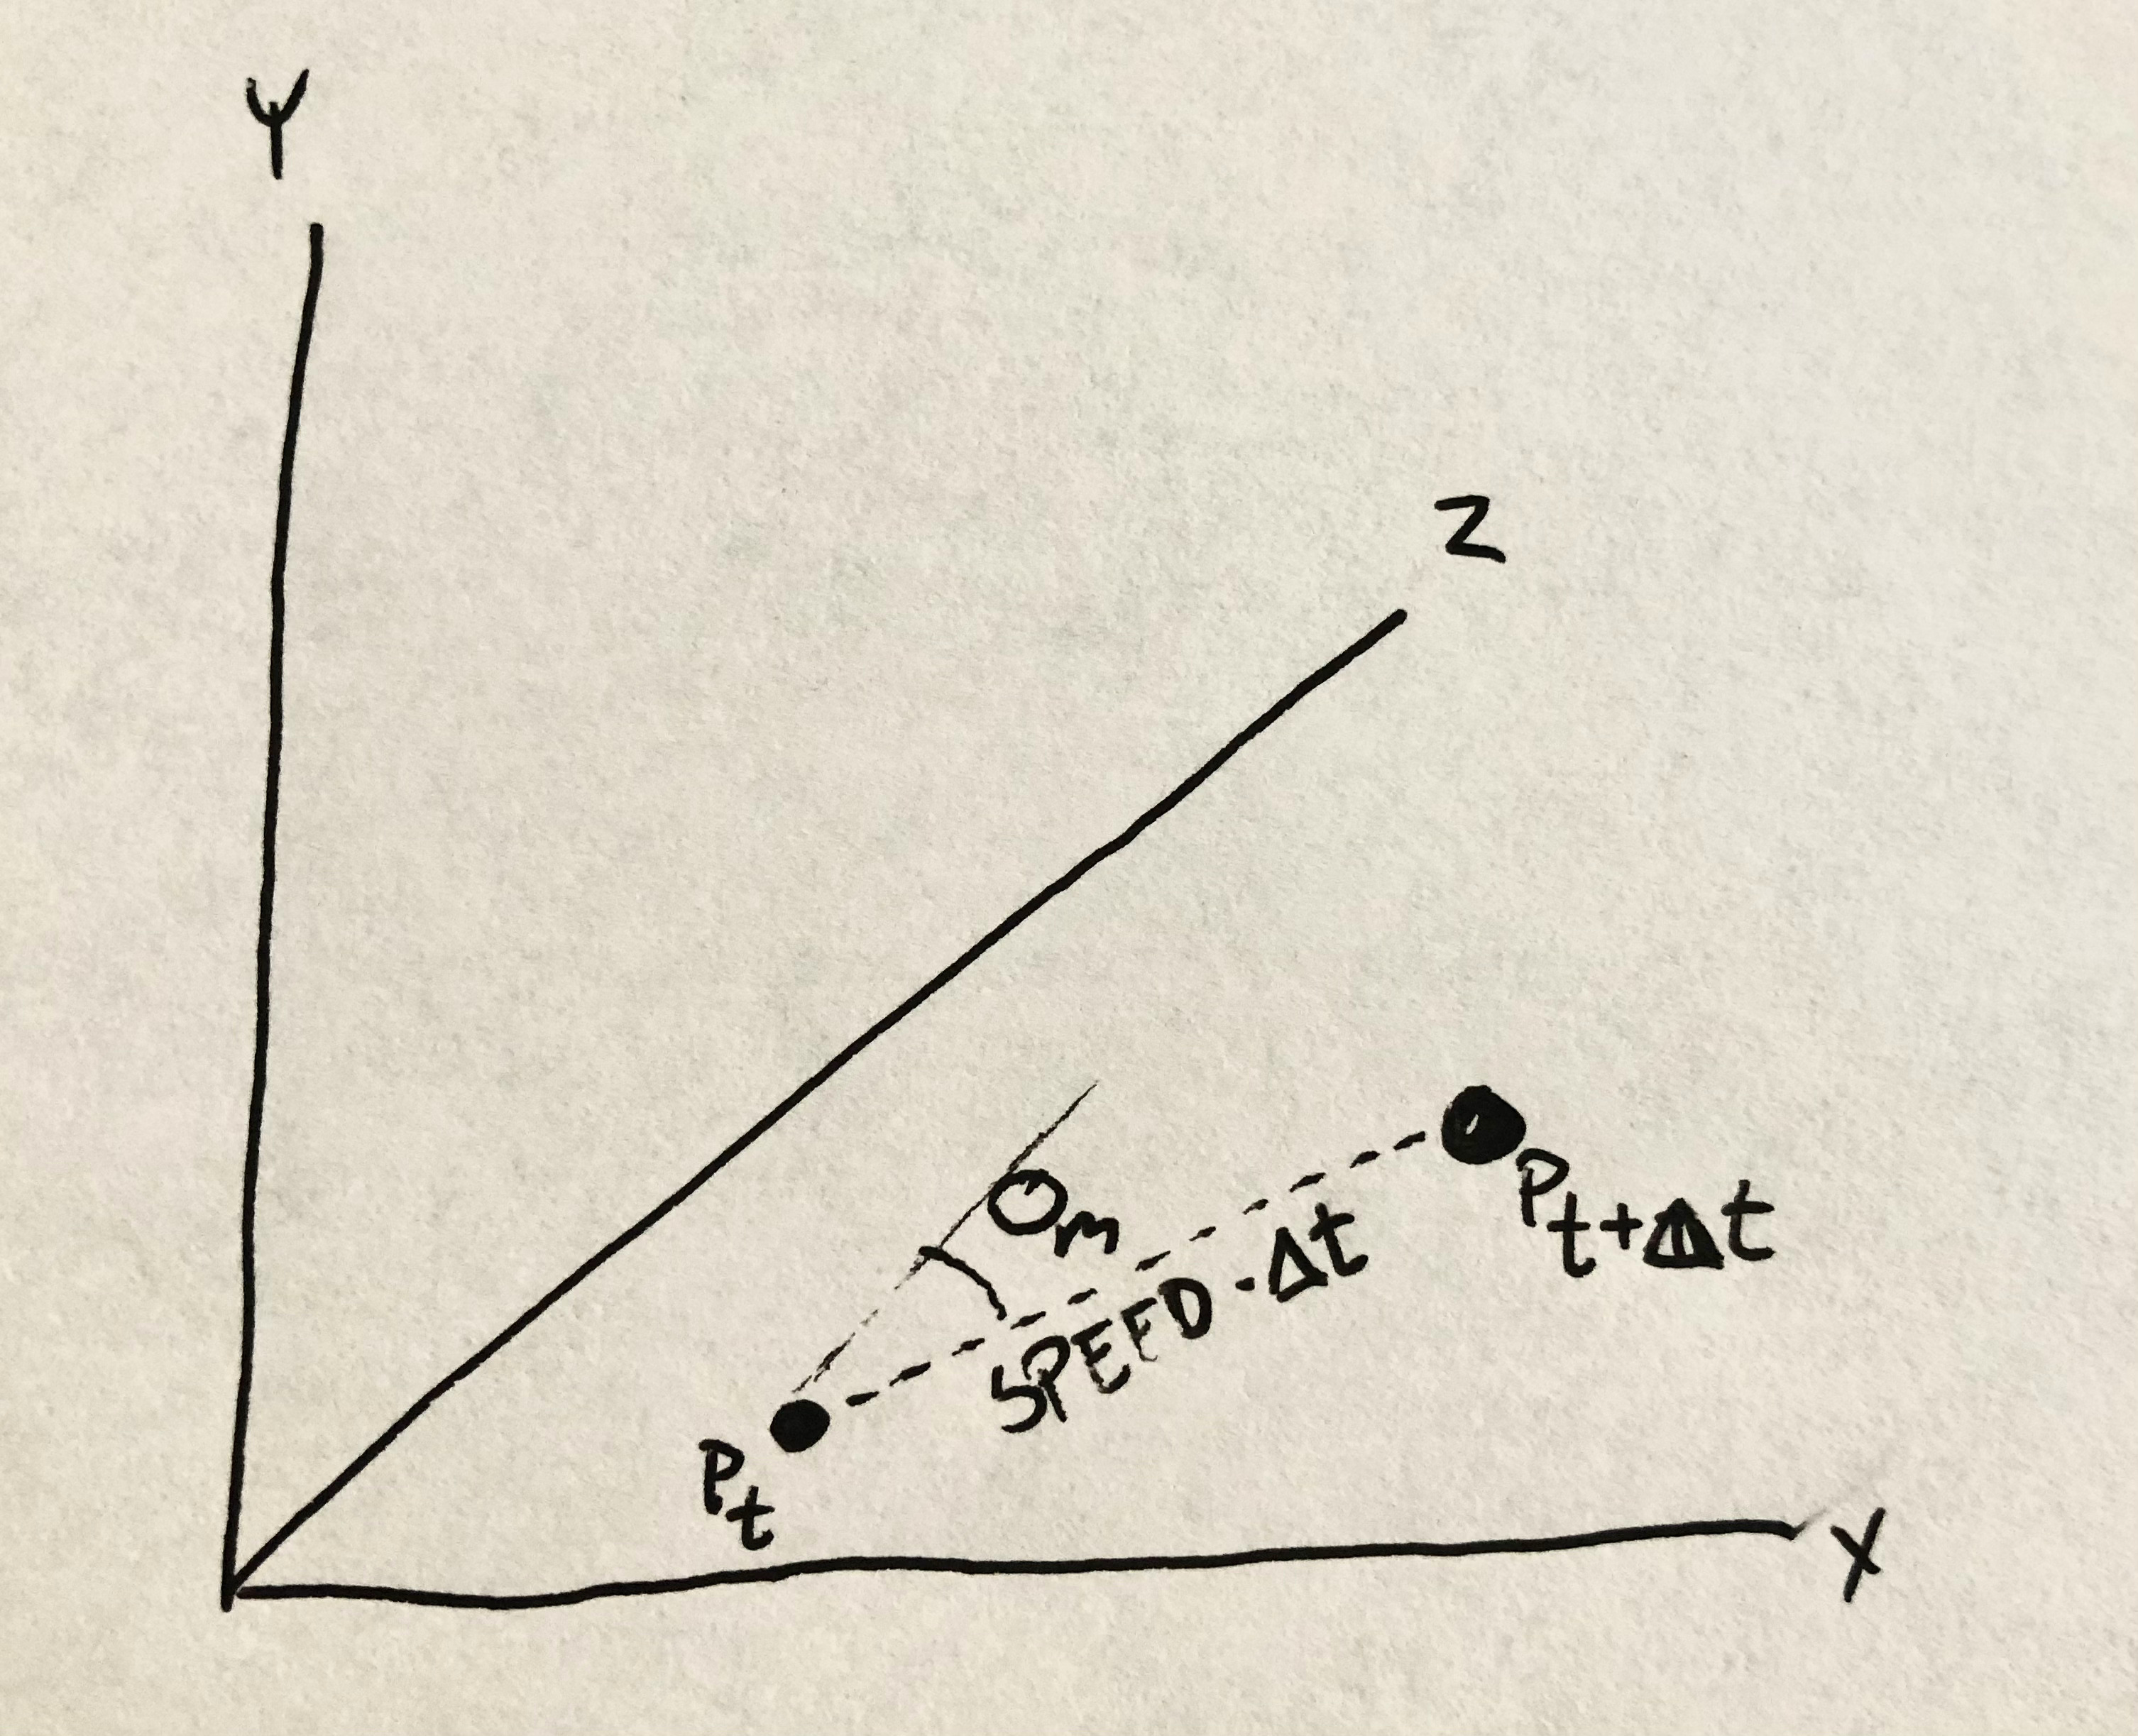
\includegraphics[width=0.75\columnwidth]{img/actor.jpg}
    \caption{Actor. Not showing derivatics and facing orientation}
    \label{fig:actor}
\end{figure}
\kenny{To make this more concrete one can for example think of $\pos$ as the planar 2D position of the character root position in the world and $\ori$ could be the world facing direction of the character given as an angle measure in the 2D world plane.} The contribution weights for different movement modes are given by the vector $\blend \equiv \begin{bmatrix}\weight_1 & \ldots & \weight_n \end{bmatrix}^T$ that contains the contribution weights $\weight_l$ for $l \in \modes$. We use the convention that $\norm{\blend}^2 = 1$ and remark that usually only a couple of modes will be active as in a transition between walking and running where 
\begin{equation}
    \label{eq:contribusion:weight:example}
    \weight_l \equiv
    \begin{cases}
    0.8 & \text{if $l$ is walking} \\
    0.2 & \text{if $l$ is running} \\
    0 & \text{otherwise}
    \end{cases}\,.
\end{equation}
To describe changes in $\blend$ over time $\dt$ each $\interpolator \in \interpolators$ defines a mapping. 
\begin{equation}
\dweight_{a} \leftarrow\interpolator_{a,b}(\weight_{b}, \dt)
\end{equation}
where $\dweight_{b}=-1*\dweight_{a}$.

The locomotion modes and interpolators are activated through high level goals provided by user control input or an AI navigation system. The goals contain no motion planning and should provide only states that we wish to achive as fast a possible. Goals are highly context dependent, and for locomotion in the plane we use the following.
\begin{subequations}
\begin{align}
     \goals &\equiv \seq{\mode_g, \kine_g} \label{eq:goals:def} \\
\end{align}
\end{subequations}

where $\mode_g$ and $\kine_g$ is the desired locomotion mode and kinematics respectively. We also use $g$ as subscript for blend weights of the requested locomotion mode.

The sparsity of the goal specifiction illustrates an inherent uncertainty in character animation, as we are challenged to infer a detailed path of movement through often complex environments given a very limited disambiguation or hints to the desired trajectory \cite{holden.ea16}. We notice that a sampling of the immediate surroundings could potentially be added as part of the goals as in \cite{holden.ea17}. 

A step of the actor state can be described by $\actor_{t+1} = step_{\actor}(\actor, \modes, \interpolators, \goals)$ and split into two separate functions to make the update process clearer.
\begin{subequations}
\begin{align}
    \blend_{t+1} &\leftarrow \sfunc_{\blend}( \blend_{t}, \interpolators, \mode_g, \dt) \label{eq:step:interpolators}\\
    \kine_{t+1} &\leftarrow  \sfunc_{\kine}(\blend_t, \kine_{t},  \modes, \kine_{g}, \dt )\label{eq:step:kinematics}
\end{align}
\end{subequations}
Where $\dt$ is a time step. Intuitively $\sfunc_{\blend}$ moves $\blend$ towards $w_g=1$ and $w_{i\neq{g}}=0$ using the combined interpolation rules in $\interpolators$. Since multiple interpolators can be active at the same time, we set the contribution of $\interpolator_k$ as the weight relative to the weight of all locomotion modes we are interpolating out of. 
\begin{equation}
\theta_{k}=\dfrac{\weight_k}{\left(\sum_{j\in\interpolators}\weight_j\right)-\weight_g}
\end{equation}
The weighted effect of all interpolators becomes.
\begin{equation}
\dweight_g = \sum_{\interpolator_j^{a\rightarrow g} \in \interpolators}\theta_a \, \interpolator_j^{a\rightarrow g}(\weight_j,\dt),
\quad \forall a \neq g \,.
\end{equation}
We set $\weight_{g,t+1}=\weight_{g,t}+\dweight_g$ and need to maintain both $||\blend||=1$ and the distribution of locomotion modes we are transitioning away from by. Both is achieved by.
\begin{equation}
\weight_{k,t+1} = \theta_k * (1-\weight_{g,t+1})  
\end{equation}

This is the general framework. Now we define locomotion modes and transitions. An actual implementation of the movement model

For $\sfunc_{\vec \omega}$ to keep the transitions defined in $\Delta{t}_c$ updates, each $\interpolator\in\interpolators$ should define a mapping $\Delta{t} \rightarrow \Delta \interp$ which also describes the duration of that transition since $\interp=1$ implies a completed interpolation. Each individual $t$ can be modelled uniquely or in a unified approach, using animator supplied curves, Sigmoids, linear interpolation or even a neural network to capture more subtleties in the transitions. In the case of transitions that are interrupted, we simply freeze existing transitions, and perform the incoming transition as a weighted combination of multiple transitions as shown in Figure \ref{fig:frozen-transition}. 
\begin{figure}
    \centering
    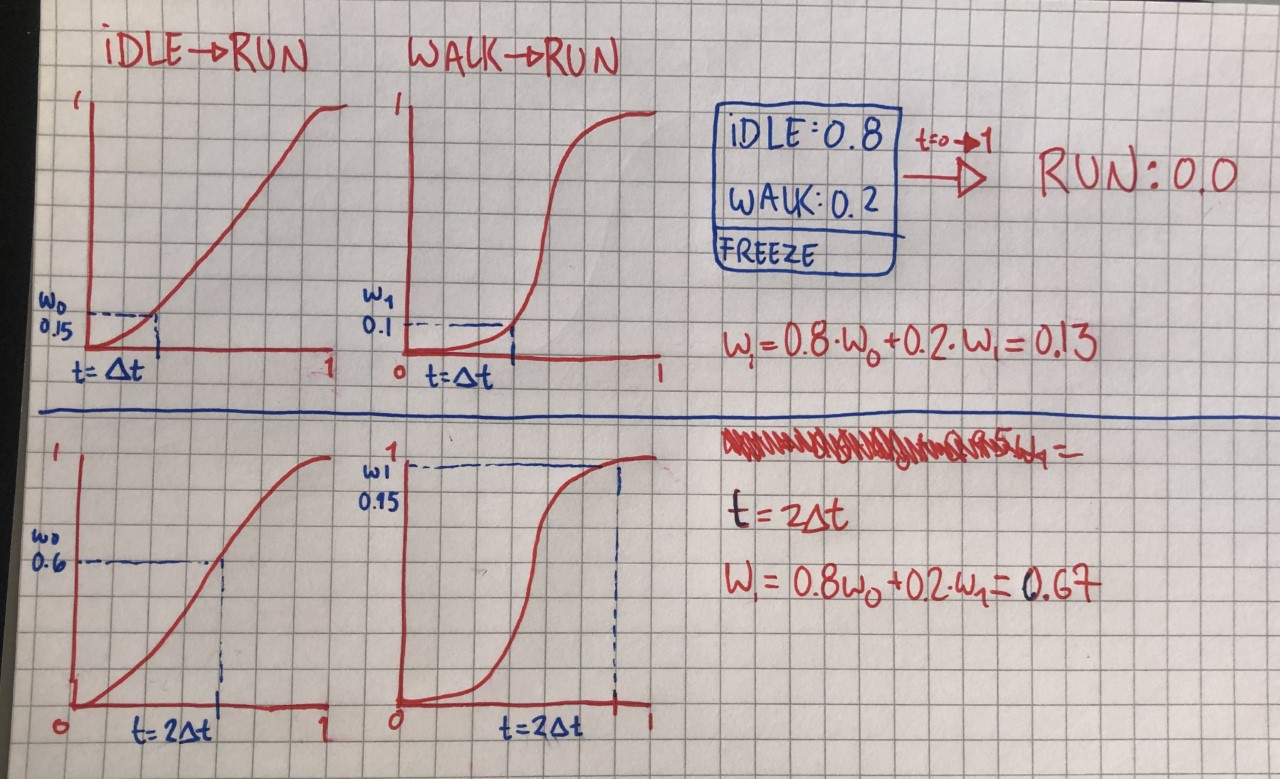
\includegraphics[width=0.75\columnwidth]{img/frozen-transitions}
    \caption{Frozen transition \kenny{Describe the take home message that reader should get from the figure}.}
  \label{fig:frozen-transition}
\end{figure}

By freezing and combining transitions in the case of interruptions, we are effectively approximating missing areas of the locomotion mode manifold by interpolations. This could be avoided by expanding $\interpolators$ to also contain transitions between combination of locomotion mode, or by expanding $\modes$ for a wider sampling of the manifold.

To evaluate $\sfunc$ we notice that each $\mode\in\modes$ should provide update routines $\dtpos_k^* \equiv \mode_{\pos,k}(\actor,\goals)$ and $\dtori_k^* \equiv \mode_{\ori, k}(\actor,\goals)$ which are then combined.
\begin{subequations}
\begin{align}
\dtpos^*&\leftarrow \sum_{k=1}^{m}\weight_k \,\mode_{\pos,k}(\actor,\goals)\\
\dtori^*&\leftarrow \sum_{k=1}^{m}\weight_k \,\mode_{\ori,k}(\actor,\goals)
\end{align}
\end{subequations}
\kenny{why sum over $m$ terms and not $n$ terms?}
The values can be inserted directly back into $\actor$ while $\pos$ and $\ori$ are updated with a forward Euler step \kenny{why this specific choice? why not just write: Position and orientation are time-integrated forward $\Delta t$ time,
\begin{subequations}
\begin{align}
    \pos^{t+\Delta t} &\leftarrow \pos^t + \int_{t}^{t+\Delta t} \dtpos^*\,dt \,, \label{eq:time:int:pos}\\
    \ori^{t+\Delta t} &\leftarrow \ori^t + \int_{t}^{t+\Delta t} \dtori^*\,dt\,, \label{eq:time:int:orientation}
\end{align}
\end{subequations}
where a simple forward Euler scheme suffices is our choice due to simplicity and performance.} using $\Delta{t}$. As before the update routines can be arbitrarily complex, which is natural given the idiosyncrasy of human movement. As such our choice of expressiveness in these function are imposing limits on the types of locomotion we are able to model. We use a simple yet expressive approach common to game development.   

velocity, velocity damper function, movement spring constant, orientation spring constant

velocity magnitude depends on the amount angular rotation. Slower when curving
move from current velocity to requested velocity is handled by spring.
move from orientation to requested orientation handled by soring.
Parameters are velocity, velocity damper function, velocity spring constant, orientation spring constant.


Notice that the formulation for $D$ is generic. In production a mapping between the generic movement model and a more context specific model would usually be needed. 

\subsection{missing}
Add animator constraint to model ? Example is 180. We dont start moving backwards immediately. First we rotate 90 degrees on the spot and then we start a 90 degree run to idle movement
Handle this by setting limits on rotation relative to forward movement ? Better to have a locomotion mode where velocity magnitude is 0 when facing relative to direction i < threshold.

Clear description of entire parameter set

Show very clear example. Pseudo code with idle and walk state. 



\section{Basic terminology}
Define animation database as $\mathcal{D}$

Define Movement model

Define Animation warping.


\section{Animation Warping}
We need a warping system that preserves ground truth. And some linear metric for divergence than can be scaled up from 0.


\section{Optimization Procedure}
We need some regularization to ill posed problem
\subsection{Primary movement modes}
Idea: Identify areas in the animations with cyclic movement for some duration. Cluster these segments into buckets with some threshold. We now have the velocity and number of main movement modes.
\subsection{Sparse user input}
If we allow extremely high frequency changes in the user input a wide variety of movement model configurations could follow the animation trajectory. We distribute sparse changes in user input over the animations, ie. few keypoints where we identify changes in the user input.


